%!TEX root = ../main.tex
%%%%%%%%%%%%%%%%%%%%%%%%%%%%%%%%%%
% Links:
%
% Difficulty: Companies: 
%%%%%%%%%%%%%%%%%%%%%%%%%%%%%%%%%%


%\begin{figure} \centering
%   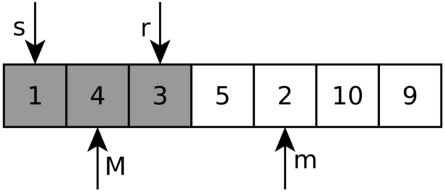
\includegraphics[width=\textwidth]{sources/max_num_chunks_sorted/images/example1}
%   \caption[Sample short cpation]{Sample Caption}. \label{fig:max_num_chunks_sorted:example1}
%   \end{figure}

\chapter{Sort the chunks, sort the array.}
\label{ch:max_num_chunks_sorted}
\section*{Introduction}

Sorting is a popular topic in computer science and programming interviews. 
Its usefulness is beyond dispute and  there are countless research papers and algorithms devoted to the topic. 

In this problem however,  we are not going to devise a novel sorting algorithm. Instead we will investigate how we can sort an entire array by sorting a number of its sub-arrays.
The idea is that we want to be able to  split an array into pieces such that if each of the pieces is sorted 
individually then the final result is equivalent to having sorted the entire array.

It is necessary to uncover a key insights  to solve this problem efficiently. 
As such, asking the right questions and looking at a certain number of good examples
is fundamental. In the next section we will explore how these insights can be gained and then turned into efficient code. 

\section{Problem statement}
\begin{exercise}
\label{example:max_num_chunks_sorted:exercice1}
Write a function that  - given an array $I$ of integers  - returns the maximum number of sub-arrays (or chunks) of $I$ 
such that , if each of the sub-array is sorted individually, then $I$ as a whole is sorted.

    %example1
    \begin{example}
        \label{example:max_num_chunks_sorted:example1}
        \hfill \\
        Given $I=\{45,88,1,9,90\}$ then the function return $1$.
        
    \end{example}

    %example2
    \begin{example}
        \label{example:max_num_chunks_sorted:example2}
        \hfill \\
        Given $I=\{4,3,2,1,5,9,10\}$ then the function return $4$. We can sort the following sub-arrays:
        \begin{itemize*}
            \item $[0,3]$
            \item $[4,4]$
            \item $[4,4]$
            \item $[4,4]$
        \end{itemize*}
    \end{example}
\end{exercise}

\section{Clarification Questions}

\begin{QandA}
    \begin{questionitem} \begin{question} Can the chunks overlap?   \end{question}      
    \begin{answered}
        \textit{No. If you choose to sort two sub-arrays of $I$ $s_1=[p,q], p\leq q$ and $s_2=[x,y], x\leq y$ then either $x > q$ or $p>y$.}
    \end{answered} \end{questionitem}
    
\end{QandA}

\section{Discussion}
\label{max_num_chunks_sorted:sec:discussion}

\section{Brute-force}
\label{max_num_chunks_sorted:sec:bruteforce}


Let's start our discussion by considering a brute-force solution. 
One possible approach would be to try to divide the array into $|I|$ non-empty and non-overlapping parts (only one way of performing such division), 
sort  them individually and then check if $I$ is sorted. 
If it is not, then we can try to divide $I$ into $|I|-1$ sub-arrays,
and check whether by sorting the resulting individual pieces $I$ turns out to be sorted.
This line of reasoning can be generalized producing a general brute-force approach
that works by progressively trying to split $I$ into less and less numbers of sub-arrays $k <|I|$.
For each of the possible valid divisions of $I$ into $k$ sub-arrays, we can then check whether we can obtain a complete sorting of $I$ by only sorting the individual $k$ sub-arrays.
Eventually when $k=1$, $I$ would be fully sorted as this is equivalent to sorting $I$ entirely.

Clearly this algorithm is complete and correct
as all possible valid partitions of $I$ are checked. Its complexity is however exponential
in time as, given a certain $k$,  there are ${n \choose k} $ possible ways we can divide $I$ into $k$ sub-arrays. 
Listing \ref{list:max_num_chunks_sorted:bruteforce} shows a C++ implementation of such idea. 



    \lstinputlisting[language=c++, caption={Bruteforce solution to the problem \textit{Sort the chunks, sort the array}.},label=list:max_num_chunks_sorted:bruteforce]{sources/max_num_chunks_sorted/max_num_chunks_sorted_solution1.cpp}



\section{Linear time}
\label{max_num_chunks_sorted:sec:lineartime}
This problem can be sorted in linear time if we consider that if we sort a sub-array of $I$
containing elements from index $s$ to $r< |I|-1$  (there is at least an element after this sub-array) 
then $I$ cannot be fully sorted if the maximum element among the elements $I_s, I_{s+1},\ldots, I_r$
is smaller than any of the elements of $I$ after $r$ (or smaller than the smallest among those elements after $r$). 
For instance, imagine $I$ is the input array of the example \ref{example:max_num_chunks_sorted:example2}. 
If we choose $s=0$ and $r=2$ then $I$ can never be properly sorted, no matter how we divide the elements after the one at index $r=2$ into subarrays
because the element at index $3$ will always appear after the value $4$ (see Figure \ref{fig:max_num_chunks_sorted:example1}).

\begin{figure}
  \centering
   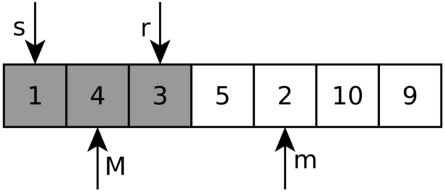
\includegraphics[width=0.6\textwidth]{sources/max_num_chunks_sorted/images/example1}
   \caption[]{Input array from the Example \ref{example:max_num_chunks_sorted:example1}. If the 
   sub-array identified by $s$ and $r$ is sorted in isolation, $I$ as a whole cannot be sorted (no matter how elements from $r$ to $|I|-1$ are sorted)
   because $M$ will always appear before $m$, despite the fact $M>m$ and it should appear after.}.
   \label{fig:max_num_chunks_sorted:example1}
\end{figure}

This insight makes it possible to derive a greedy approach to this problem that is based on the idea that we 
are going to split $I$ into as many pieces as possible, such that the largest element of a sub-array 
is smaller than all the subsequent elements. 

Listing \ref{list:max_num_chunks_sorted:linear} shows an implementation of this that works by keeping a sorted list $N$
of all the elements not yet processed in $I$. $N$ initially contains all the values in $I$.
We start a new chunk at index $0$ and we keep including elements into this chunk until the largest
of its elements is still larger than the smallest element in $N$.
When an element is included in the chunk then it is removed from $N$.
If the largest element in the current chunk is indeed smaller than the smallest in $N$,
then this signals the fact we can sort this chunk independently without
causing $I$ as a whole not to be sorted (all the elements of this chunk appear before the rest of the elements when $I$ is sorted).
At this point, we can start a new chunk and repeat the process until
we are left with no element to process (or equivalently $N$ is empty).
Listing \ref{list:max_num_chunks_sorted:linear} has a complexity of $O(|I|)$ for both space and time. 

\lstinputlisting[language=c++, caption={Linear time solution to the problem \textit{Sort the chunks, sort the array}.},
    label=list:max_num_chunks_sorted:linear]{sources/max_num_chunks_sorted/max_num_chunks_sorted_solution2.cpp}